\subsection{Student Landing Page}

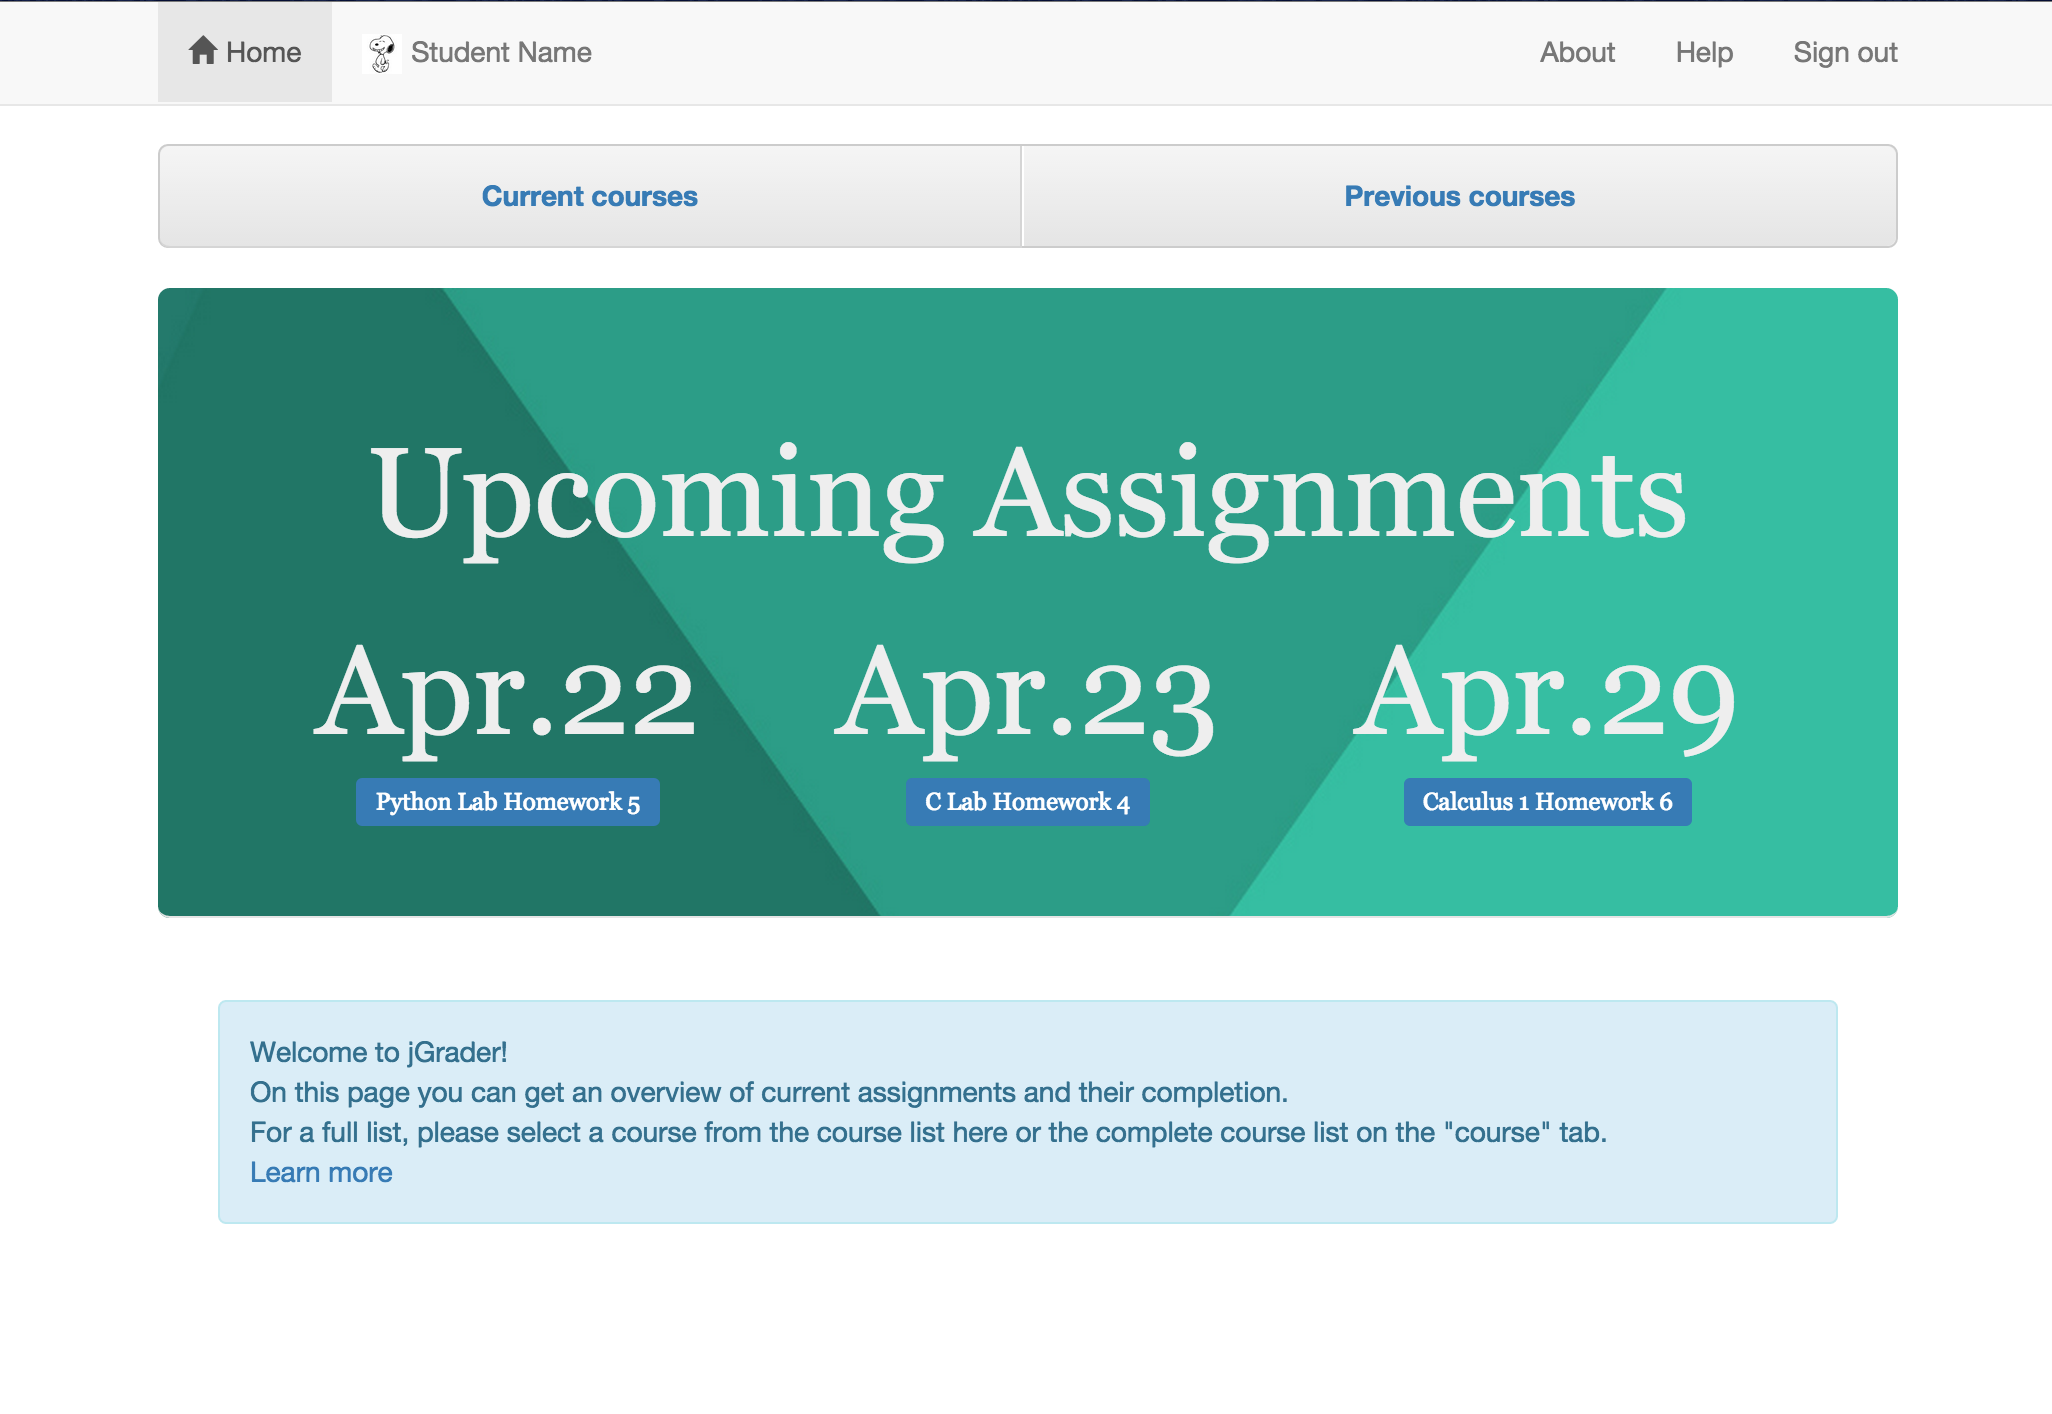
\includegraphics[width=\textwidth]{screenshots/StudentUpcomingAssignments.png}

\begin{itemize}

\item Students are provided with an overview of upcoming deadlines and how much of the tasks are done (e.g. if the student finished 4 out of 5 tasks it will visually show 80\%). This will help students remember all their deadlines.

\item Links on the visual representation of the percentages will allow students to quickly navigate to the assignments that are due.

\item To limit the information that is on the screen previous courses are only shown when the student clicks on the rider for previous courses. This ensures that the page provides an easily processable overview without clutter.

\item In the Enrolled Courses section, the student can access all courses he is currently enrolled in.

\end{itemize}
